% This must be in the first 5 lines to tell arXiv to use pdfLaTeX, which is strongly recommended.
\pdfoutput=1
% In particular, the hyperref package requires pdfLaTeX in order to break URLs across lines.

\documentclass[11pt]{article}

\usepackage[review]{acl}
\usepackage{times}
\usepackage{latexsym}
\usepackage[T1]{fontenc}
\usepackage[utf8]{inputenc}
\usepackage{microtype}
\usepackage{inconsolata}
\usepackage{booktabs}
\usepackage{multirow}
\usepackage{subfiles}
\usepackage{graphicx}
\usepackage{colortbl}

% Commands 
\newcommand{\draftonly}[1]{#1}
\newcommand{\draftcomment}[3]{\draftonly{\textcolor{#2}{[#3]{$_{\textsc{#1}}$}}}}
\newcommand{\lj}[1]{\draftcomment{Lj}{red}{#1}}
\newcommand{\libertus}{\textsc{LiBERTus}}


\title{Team 21a's Submission to the SIGTYP 2024 Shared Task on Word Embedding Evaluation for Ancient and Historical Languages}

\author{Lester James V. Miranda \\
  Allen Institute for Artificial Intelligence \\
  \texttt{ljm@allenai.org} \\
}

\begin{document}

\maketitle

\begin{abstract}
In this paper, we describe Team 21a's submission to the constrained track of the SIGTYP 2024 Shared Task.
Using only the data provided by the organizers, we pretrained a transformer-based multilingual model, then finetuned it on the Universal Dependencies (UD) annotations of a given language for a downstream task.
We also explored the cross-lingual capability of our trained models.
\lj{Our systems achieved}
% TODO: talk about results and scores on the test set
% maybe benchmark against XLM-RoBERTa and mBERT just for a good baseline?
\end{abstract}

\section{Introduction}
This paper describes Team 21a's submission to the \textit{constrained} track of the SIGTYP 2024 Shared Task on Word Embedding Evaluation for Ancient and Historical Languages.
Our general approach involves pretraining a transformer-based multilingual model on the shared task dataset, and then finetuning the pretrained model using the Universal Dependencies (UD) annotations of each language.
Throughout this paper, we will refer to the pretrained model as \libertus{}.
We also explored data sampling and augmentation techniques during the pretraining step to ensure better generalization performance.

Our systems achieved...\lj{stuff}. 
Table \ref{table:main_results} shows our systems' performance on the shared task test set.


We detail our resource creation, model pretraining, and finetuning methodologies.
The source code for all experiments can be found on GitHub: \lj{insert github link or OSF link for anonymity}.

\subfile{tables/main_results.tex}

\section{Methodology}

% We noticed that there is a stark diffence in token distribution across all languages, so we used an upsampling strategy to balance them out.
% Figure \ref{fig:unique_tokens} shows that \textsc{latm} has the most number of unique tokens in the corpora.
% We upsampled each language by randomly duplicating a document in the training pool until the number of unique tokens (with allowance for duplicates) is greater than or equal to that of \textsc{latm}.
% The same figure also shows the token counts after the augmentation process.

% \begin{figure}[t]
% \centering
% 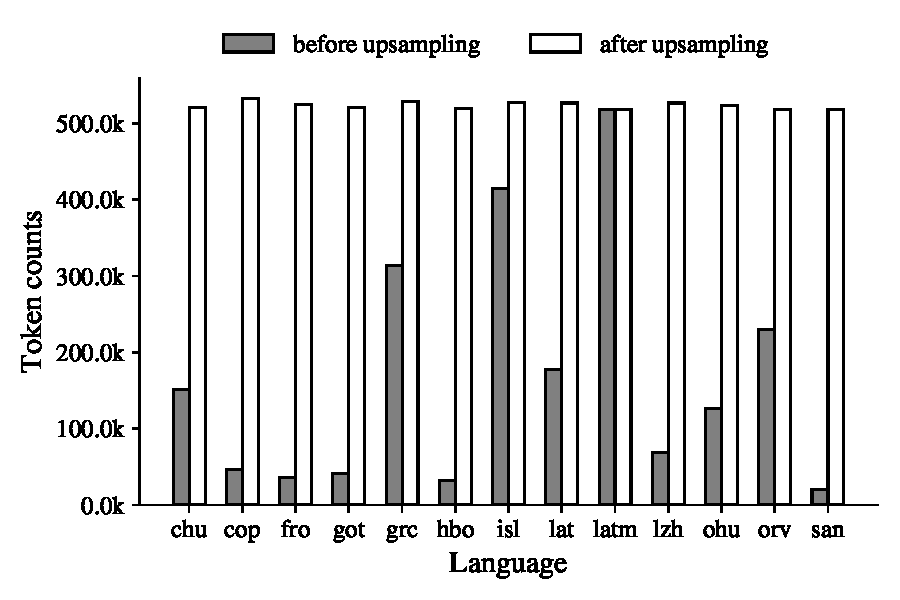
\includegraphics[width=0.5\textwidth]{figures/token_counts.pdf}
% \caption{Unique token counts (with allowance for duplicates) for each language before and after upsampling.}
% \label{fig:unique_tokens}
% \end{figure}

\subsection{Model Pretraining}

\begin{figure}[t]
\centering
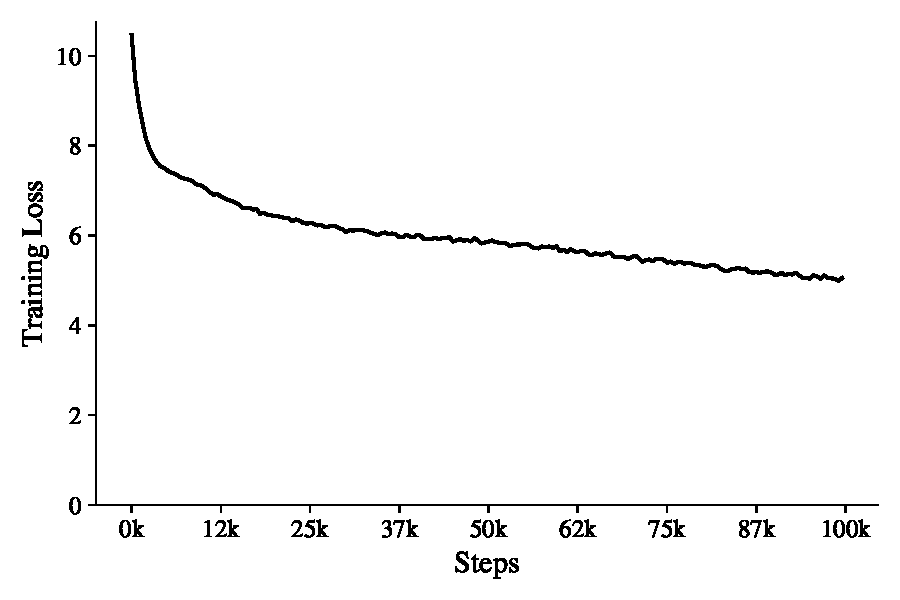
\includegraphics[width=0.5\textwidth]{figures/train_loss.pdf}
\caption{Training loss curve for the 126M-parameter model after 100k steps.}
\label{fig:training_curve}
\end{figure}

\paragraph{Preparing the pretraining corpora.} We constructed the pretraining corpora using the annotated tokens of the shared task dataset.
Then, we explored several data augmentation techniques to ensure that each language is properly represented based on the number of unique tokens.
Initially, we upsampled each language to match the token count of \textsc{latm} (highest unique token count), but we found that the training loss jumps up by 5-pp in the middle of pretraining.

In the end, we found that leaving the token distribution as-is leads to more stable pretraining and lower validation scores.

\paragraph{Pretraining the base model.} Using the pretraining corpora, we trained a model with 126M parameters that will serve as a base for finetuning downstream tasks.
\libertus{} follows RoBERTa's pretraining architecture \cite{liu-etal-2019-roberta} and takes inspiration from \citet{conneau-etal-2020-unsupervised}'s work on scaling BERT models to multiple languages.

\subfile{tables/pretrain_hyperparams.tex}

Our hyperparameter choices closely resemble that of the original RoBERTa implementation as seen in Table \ref{table:pretrain_hyperparams}.
We also trained the same BPE tokenizer \citep{sennrich-etal-2016-neural} using the constructed corpora.
During model pretraining, we used the AdamW optimizer with $\beta_2$=0.98 and a weight decay of 0.01.
The base model underwent training for 100k steps with a learning rate of 2e-4.
We used a learning rate scheduler that linearly warms up during the first 12k steps of the training process, then linearly decays for the rest.
Figure \ref{fig:training_curve} shows the training curve.

\subsection{Model Finetuning}

For each language, we finetuned a multitask model using spaCy \cite{honnibal-etal-2020-spacy}. 
The final system consists of a parts-of-speech (POS) tagger, morphological analyzer, and lemmatizer.

\paragraph{Parts-of-speech (POS) tagger.}
We employed a standard classifier that predicts a vector of tag probabilities for each token.
Each POS tag is a unique class that we assign exclusively to a token.
We trained a model by taking the context-sensitive vectors from our pretrained embeddings, and passing it to a linear layer with a softmax activation.
The network is then optimized using a categorical cross-entropy loss.

\paragraph{Morphological analyzer.}
Similar to the POS tagger, we treat morphological annotation as a token classification task.
Instead of directly modeling each feature, we made every unique combination of morphological features as a class.
The limitation of this approach is that it can only predict combinations that were present in the training corpora.

\begin{figure*}[t]
\centering
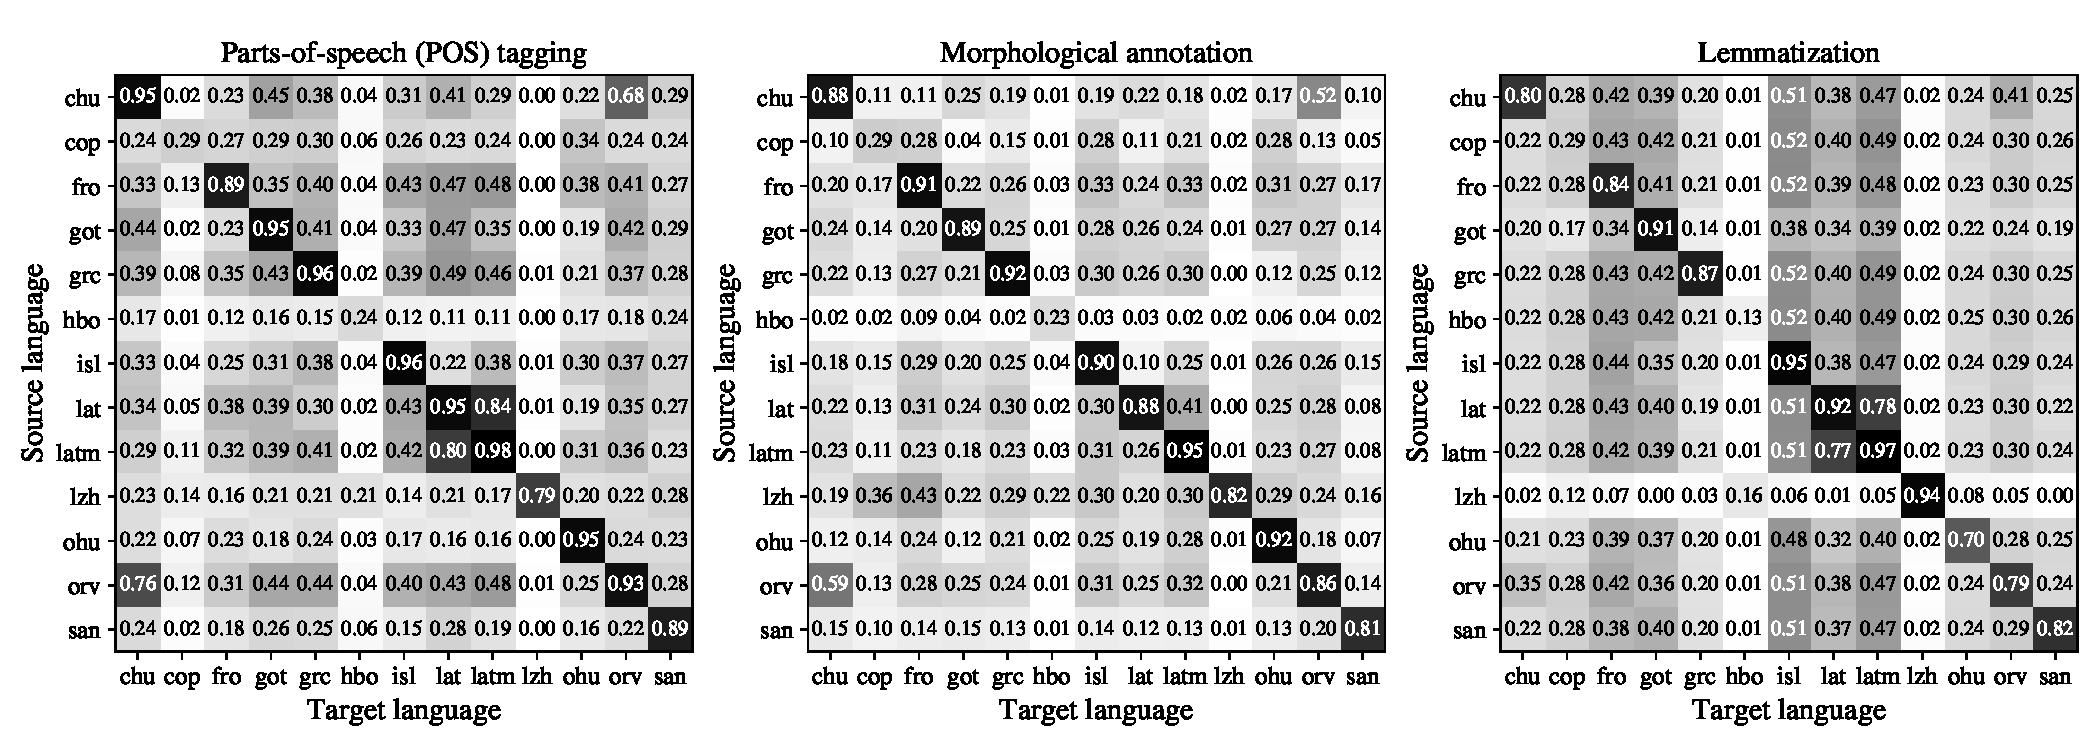
\includegraphics[width=\textwidth]{figures/cross_lingual.pdf}
\caption{Cross-lingual evaluation given a monolingual model from one language and a validation set in another.}
\label{fig:cross_lingual}
\end{figure*}


\paragraph{Lemmatizer.} 
We trained a neural-based edit tree lemmatizer \cite{muller-etal-2015-joint} by first extracting an edit tree for each token-lemma pair.
Because this process can result to hundreds of edit trees, we treat the problem of picking the correct tree as a classification task.
Here, each unique tree serves as a class and we compute a probability distribution over all trees for a given token.
To obtain the most probable tree, we passed the context-sensitive embeddings from our pretrained model to a softmax layer and trained the network with a cross-entropy loss objective.

We set the minimum frequency of an edit tree to 3, and used the surface form of the token as a backoff when no applicable edit tree is found.
Finally, we ensured that the lemmatizer checks at least a single tree before resorting to backoff. \\

\noindent We trained each component of the system in parallel, although the final ``pipeline'' assembles them together using the spaCy framework.
For all components, the pretrained embeddings are passed on to linear layer with softmax activation.
Sometimes, the tokenization from the multilingual model does not align one-to-one with spaCy's tokenization.
In such case, we use a pooling layer that computes the average of each feature to obtain a single vector per spaCy token.

During finetuning, we used the Adam optimizer with $\beta_1$=0.9, $\beta_2$=0.999 and a learning rate of $0.001$.
The learning rate warms up linearly for the first 250 steps, and then decays afterwards.

\section{Results}

Table \ref{table:main_results} shows the test scores for the shared task.
\lj{Talk about how you ranked against other teams?}
In this section, we will outline our internal evaluations and benchmarking experiments.



\subsection{Performance on the validation set}

\subfile{tables/validation_results.tex}

First, we evaluated our finetuned models on the validation set.
Table \ref{table:validation_results} shows the results.
Although we obtained strong performance on the majority of languages, our results on \textsc{cop}, \textsc{hbo}, and \textsc{lzh} are poor.
These languages have non-latin scripts, and our tokenizer cannot handle these characters.
In the end, we decided to prioritize having a single multilingual model for the task so we maintained our tokenizer choice.

\subsection{Evaluating cross-lingual capabilities}
\label{sec:results_crosslingual}

To test the cross-lingual capability of a language, we evaluated its finetuned model to the validation set of another.
Figure \ref{fig:cross_lingual} shows the results.

We found that it is possible to adapt a language onto another for morphological annotation and lemmatization.
However, this does not extend to POS tagging, as the validation set performs best only in the language it was trained on.

Some target languages tend to be cross-lingually receptive on lemmatization, i.e., many source languages can perform decently when applied to them.
This observation is true for \textsc{fro}, \textsc{got}, \textsc{isl}, \textsc{lat}, and \textsc{latm}.
Finally, there is also good cross-lingual compatibility between \textsc{lat} and \textsc{latm}\textemdash which is expected because they came from similar roots. 

\section{Conclusion}

This paper describes Team 21a's system: a pretrained multilingual model (\libertus{}) finetuned on different languages for each downstream task.
Our system obtained \lj{describe your rank, how you stack, etc. etc.}

Our system's main strength is its downstream performance.
The validation scores are high for the majority of languages.
However, it is limited by its tokenizer, resulting to poor performance on languages with non-latin scripts.
We also evaluated each language's cross-lingual capability and showed that transfer learning is possible especially on lemmatization.
This approach can be a viable alternative on limited corpora.

The source code for training and experimentation can be found on GitHub: \lj{insert GitHub or OSF url}.
We will also release the pretrained multilingual model and finetuned pipelines in public shortly after the review period.

\section*{Limitations}

\paragraph{Handling non-Latin scripts.}
The performance of our downstream models on \textsc{cop}, \textsc{hbo}, and \textsc{lzh} are below 0.5.
We believe that this is due to our tokenization method, which fails for non-latin scripts.
We encourage exploring alternative tokenization strategies that are better equipped to handle diverse script types.

\paragraph{Pretrained LM size.}
Due to compute constraints, we were only able to pretrain a model akin to the size of RoBERTa\textsubscript{base}.
We highly recommend pretraining a large \libertus{} model to obtain performance gains if the resource allows.

\paragraph{Pretraining data mix.}
In the end, we didn't employ any sampling strategy to balance the token distribution of different languages during pretraining.



\bibliography{custom}

\appendix

\section{Appendix}
\label{sec:appendix}

\subsection{Different sampling strategies on pretraining validation performance}

We explored different sampling strategies and their effect on the pretraining validation loss curve as shown in Figure \ref{fig:effect_sampling}.

\begin{itemize}
  \item \textbf{None:} we used the original dataset without any data sampling or augmentation.
  \item \textbf{Upsampling:} we upsampled each language to ensure that the number of their unique tokens is greater than or equal to the most dominant language.
  \item \textbf{Averaging:} we took the average number of unique tokens in the whole set and up-/downsampled each language based on this value.
\end{itemize}

The evaluation corpus was built from the validation set of the shared task, and we kept it the same throughout the experiment.
It is interesting that sampling is detrimental to validation loss, but in our final system, we employed the upsampling strategy as we believe that it would provide a more robust performance across all languages.


\subsection{Finetuning a model per language vs. monolithic system}

We investigated if finetuning a model per language is more effective against a monolithic system, i.e., training on the full multilingual annotated corpora.
Here, we combined the training corpora for all languages, then shuffled them before batching.
The merged dataset has 194,281 documents for training and 26,954 documents for validation.
This means that the downstream model sees a language mix per training epoch.

We found out that although more expensive, finetuning a model per language still yields the best results. 
Figure \ref{fig:full_vs_langspecific} illustrates these results.


\subsection{Alternative approach we considered}

\begin{figure*}[t]
\centering
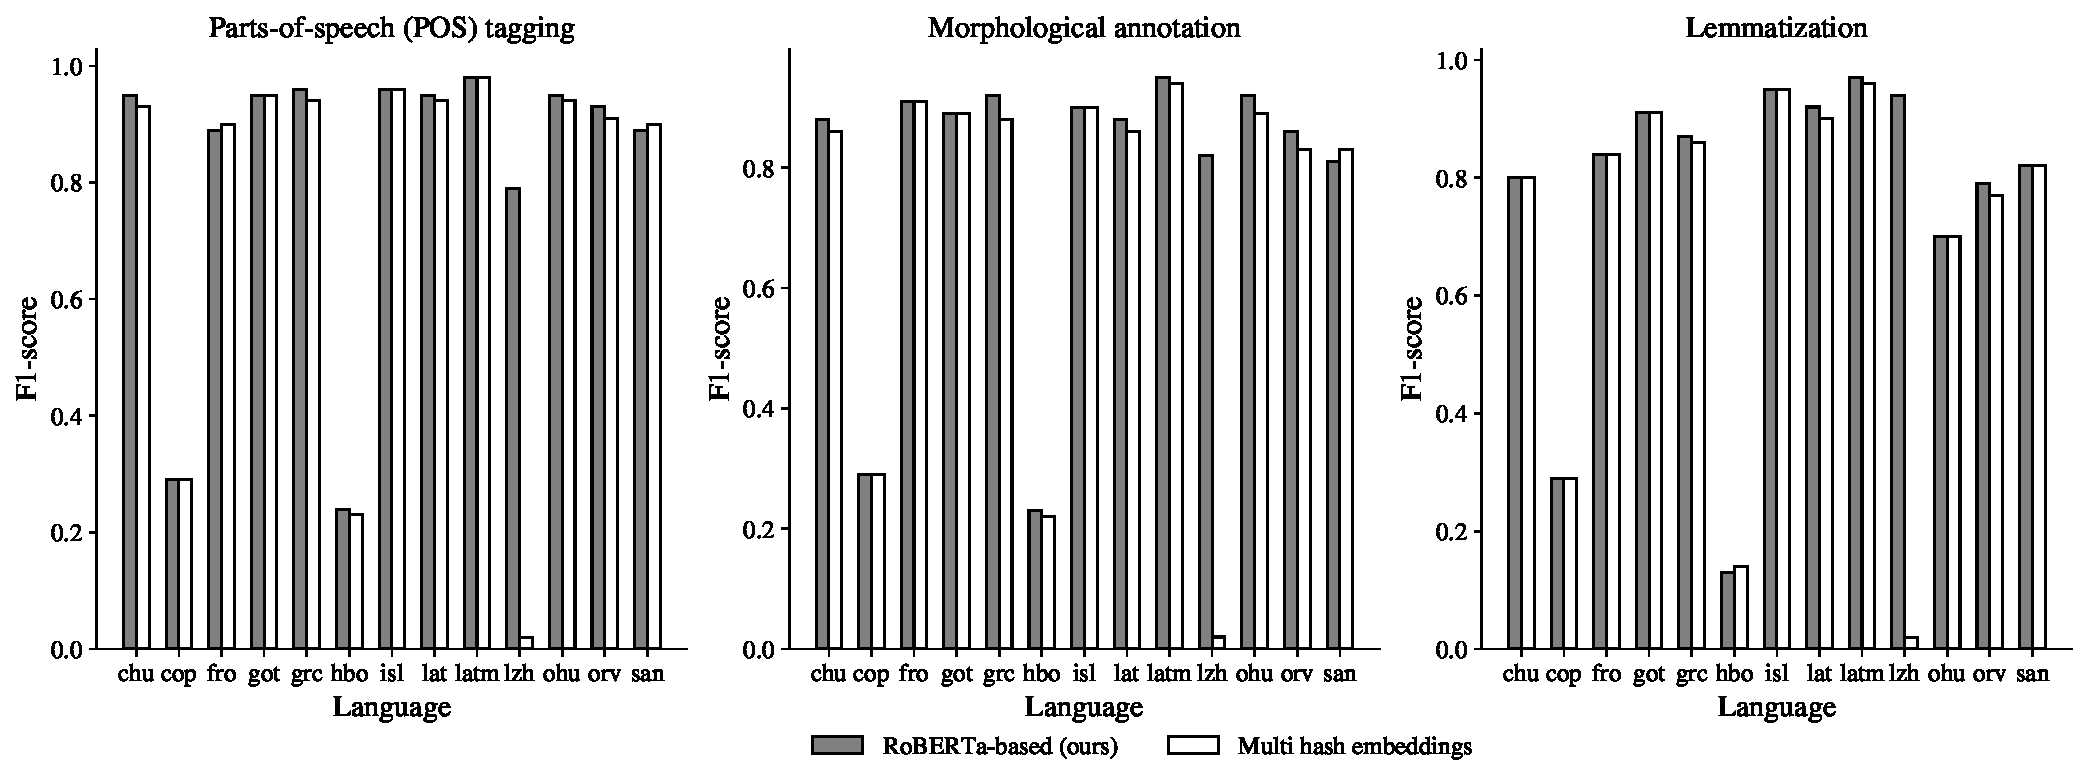
\includegraphics[width=\textwidth]{figures/hashembed.pdf}
\caption{Comparison.}
\label{fig:hashembed}
\end{figure*}

We considered using multi-hash embeddings \cite{miranda-etal-2022-multi} as an alternative approach.
Instead of pretraining, these embeddings use orthographic features (e.g., prefix, suffix, norm, shape) to create a word vector table.
This approach also applies the hashing trick, inspired by Bloom filters \cite{bloom-1970-space}, to decrease the vector table's memory footprint.

Figure \ref{fig:hashembed} shows the results in comparison to our final system.
It is notable that simple orthographic features are competitive with our transformer-based model.
However, we chose to submit the transformer-based pipeline as our final system because it still outperforms the multi-hash embed method in the majority of our language-task pairs. 
We still recommend investigating this approach further because the hash-embed method has noticeable efficiency gains in terms of model size.

\end{document}
